\documentclass[tikz,border=10pt]{standalone}
\usepackage{tikz}
\usepackage{fontawesome5}
\usepackage{amsmath,amssymb}
\usetikzlibrary{arrows.meta,positioning,fit,backgrounds,calc,shadows,shapes.geometric}

% Color definitions
\definecolor{lavenderDark}{RGB}{15, 44, 89}
\definecolor{lavenderDeep}{RGB}{10, 28, 58}
\definecolor{lavenderMedium}{RGB}{29, 78, 158}
\definecolor{lavenderLight}{RGB}{240, 246, 255}
\definecolor{lavenderBorder}{RGB}{180, 205, 237}
\definecolor{prismNavy}{RGB}{15, 44, 89}
\definecolor{prismBlue}{RGB}{29, 78, 158}
\definecolor{prismTeal}{RGB}{13, 148, 136}
\definecolor{prismMint}{RGB}{236, 253, 245}
\definecolor{prismGold}{RGB}{217, 119, 6}
\definecolor{prismDark}{RGB}{15, 23, 42}
\definecolor{prismSlate}{RGB}{100, 116, 139}
\definecolor{statusFail}{RGB}{220, 38, 38}
\definecolor{cStem}{RGB}{224, 242, 254}
\definecolor{cStage1}{RGB}{209, 250, 229}
\definecolor{cHead}{RGB}{219, 234, 254}
\definecolor{cDeliverable}{RGB}{204, 251, 241}

\begin{document}
\begin{tikzpicture}[
  x=1cm, y=1cm,
  tblcard/.style={
    rectangle, rounded corners=4pt, draw=lavenderDark!80, line width=0.85pt, fill=white,
    inner sep=5pt, text width=4.70cm, align=left,
    drop shadow={shadow xshift=1pt, shadow yshift=-1pt, opacity=0.10}
  },
  fkarrow/.style={
    -{Stealth[scale=0.95]}, line width=1.1pt, draw=lavenderDark!90
  },
  fklabel/.style={
    font=\fontsize{6.8}{8.0}\selectfont\bfseries, fill=white, inner sep=1.8pt, text=lavenderDark, draw=lavenderBorder, line width=0.5pt, rounded corners=2pt
  }
]

  % ================= COLUMN 1: VOTER & ADMIN (x = -4.5) =================
  
  % Table 1: Voter Struct
  \node[tblcard, fill=cStem!45] (voter) at (-4.5, 1.9) {%
    \centerline{\color{lavenderDark}\faUserCheck\ \textbf{\fontsize{8.5}{10.0}\selectfont struct Voter}}\\[2pt]
    \rule{\linewidth}{0.4pt}\\[2pt]
    {\fontsize{7.2}{8.8}\selectfont
    \textbf{\color{lavenderDark}[KEY]} \texttt{address}: \textit{address} (160-bit hex)\\
    \textbf{\color{prismTeal}[STATE]} \texttt{isRegistered}: \textit{bool}\\
    \textbf{\color{statusFail!90!black}[STATE]} \texttt{hasVoted}: \textit{bool} (Atomic flag)\\
    \textbf{\color{prismBlue}[FK]} \texttt{votedCandidateId}: \textit{uint}\\
    \textbf{\color{prismDark!80}[FLD]} \texttt{voteTimestamp}: \textit{uint256}}
  };

  % Table 2: Election Admin & Config
  \node[tblcard, below=0.65cm of voter, fill=cHead!45] (admin) {%
    \centerline{\color{lavenderDark}\faUserShield\ \textbf{\fontsize{8.5}{10.0}\selectfont contract ElectionState}}\\[2pt]
    \rule{\linewidth}{0.4pt}\\[2pt]
    {\fontsize{7.2}{8.8}\selectfont
    \textbf{\color{lavenderDark}[OWNER]} \texttt{admin}: \textit{address} (Contract owner)\\
    \textbf{\color{prismDark!80}[MAP]} \texttt{voters}: \textit{mapping(address $\Rightarrow$ Voter)}\\
    \textbf{\color{prismDark!80}[ARR]} \texttt{candidates}: \textit{Candidate[]}\\
    \textbf{\color{prismTeal}[CNT]} \texttt{candidatesCount}: \textit{uint}\\
    \textbf{\color{prismGold}[CNT]} \texttt{totalVotesTallied}: \textit{uint256}}
  };

  % ================= COLUMN 2: CANDIDATE & LEDGER RECEIPT (x = 4.5) =================

  % Table 3: Candidate Struct
  \node[tblcard, fill=cStage1!45] (candidate) at (4.5, 1.9) {%
    \centerline{\color{lavenderDark}\faVoteYea\ \textbf{\fontsize{8.5}{10.0}\selectfont struct Candidate}}\\[2pt]
    \rule{\linewidth}{0.4pt}\\[2pt]
    {\fontsize{7.2}{8.8}\selectfont
    \textbf{\color{lavenderDark}[PK]} \texttt{id}: \textit{uint} (Unique candidate ID)\\
    \textbf{\color{prismDark!80}[FLD]} \texttt{name}: \textit{string} (Candidate Moniker)\\
    \textbf{\color{prismTeal}[TALLY]} \texttt{voteCount}: \textit{uint} (Total $N(c)$)\\
    \textbf{\color{prismBlue}[AUDIT]} \texttt{registrationBlock}: \textit{uint256}\\
    \textbf{\color{prismGold}[VAL]} \texttt{isValid}: \textit{bool}}
  };

  % Table 4: Transaction & Event Receipt
  \node[tblcard, below=0.65cm of candidate, fill=cDeliverable!55] (receipt) {%
    \centerline{\color{lavenderDark}\faReceipt\ \textbf{\fontsize{8.5}{10.0}\selectfont event VoteCast \& Receipt}}\\[2pt]
    \rule{\linewidth}{0.4pt}\\[2pt]
    {\fontsize{7.2}{8.8}\selectfont
    \textbf{\color{lavenderDark}[HASH]} \texttt{txHash}: \textit{bytes32} (Keccak-256)\\
    \textbf{\color{prismBlue}[IDX]} \texttt{voter}: \textit{address} (Indexed sender)\\
    \textbf{\color{prismTeal}[IDX]} \texttt{candidateId}: \textit{uint} (Indexed choice)\\
    \textbf{\color{prismDark!80}[BLK]} \texttt{blockNumber}: \textit{uint256}\\
    \textbf{\color{prismGold}[SEAL]} \texttt{blockHash}: \textit{bytes32}}
  };

  % Foreign Key & Relational Connectors
  \draw[fkarrow] (voter.east) -- (candidate.west)
    node[midway, fklabel] {votes for candidateId};

  \draw[fkarrow] (admin.north) -- (voter.south)
    node[midway, fklabel] {manages whitelist};

  \draw[fkarrow] (admin.east) -- (candidate.south west)
    node[pos=0.40, fklabel, sloped] {registers Candidate};

  \draw[fkarrow] (admin.east) -- (receipt.west)
    node[midway, fklabel] {emits VoteCast};

  \draw[fkarrow] (candidate.south) -- (receipt.north)
    node[midway, fklabel] {increments voteCount};

\end{tikzpicture}
\end{document}
